\chapter{Combinatorial Analysis}

\section{Why combinatorial analysis?}

A communication system consist of \(n\) seemingly identical antennas that are lined up in a linear ordered array. The resulting system will then be able to receive all incoming signals and will be called functional as long as no two consecutive antennas are defective. If \(m\) of the \(n\) antennas are defective, how many different states of the system are possible?

If \(n =4\) and \(m=2\) there are \(6\) states possible : 

\[ 
\begin{matrix}
    0 & 1 & 1 & 0 \\
    1 & 0 & 1 & 0 \\
    1 & 0 & 0 & 1 \\
    0 & 1 & 0 & 1 \\
    0 & 0 & 1 & 1 \\
    1 & 1 & 0 & 0 \\
\end{matrix}
\]

In \(6\) of these \(3\) of them are functional. 

\begin{definition}
    The mathematical theory of counting is known as \textbf{combinatorial analysis}  
\end{definition}

\section{The basic principle of counting}

\begin{definitionbox}[title=The Basic Principle of Counting]
    Suppose that two experiments are to be performed. The first experiment has \(m\) possible outcomes and for each of these outcomes the second experiment has \(n\) possible outcomes. Then the two experiments together have \(m \times n\) possible outcomes.
\end{definitionbox}
\begin{examplebox}[title=Example: Coin and Die]
    A coin is tossed and a die is rolled. How many possible outcomes are there?
    
    \textbf{Solution:} The coin has \(2\) possible outcomes and the die has \(6\) possible outcomes. Therefore the two experiments together have \(2 \times 6 = 12\) possible outcomes.
\end{examplebox}


\begin{definitionbox}[title=The Generalized Basic Principle of Counting]
    If \(r\) experiments are to be performed are to be such that the first one may result in any of \(n_1\) possible outcomes, and for each of these \(n_{1}\) possible outcomes there are \(n_2\) possible outcomes for the second experiment, and so on up to the \(r\)-th experiment which may result in any of \(n_r\) possible outcomes, then the \(r\) experiments together have \(n_1 \times n_2 \times \ldots \times n_r\) possible outcomes.
\end{definitionbox}


\begin{figure}[H]
    \centering
    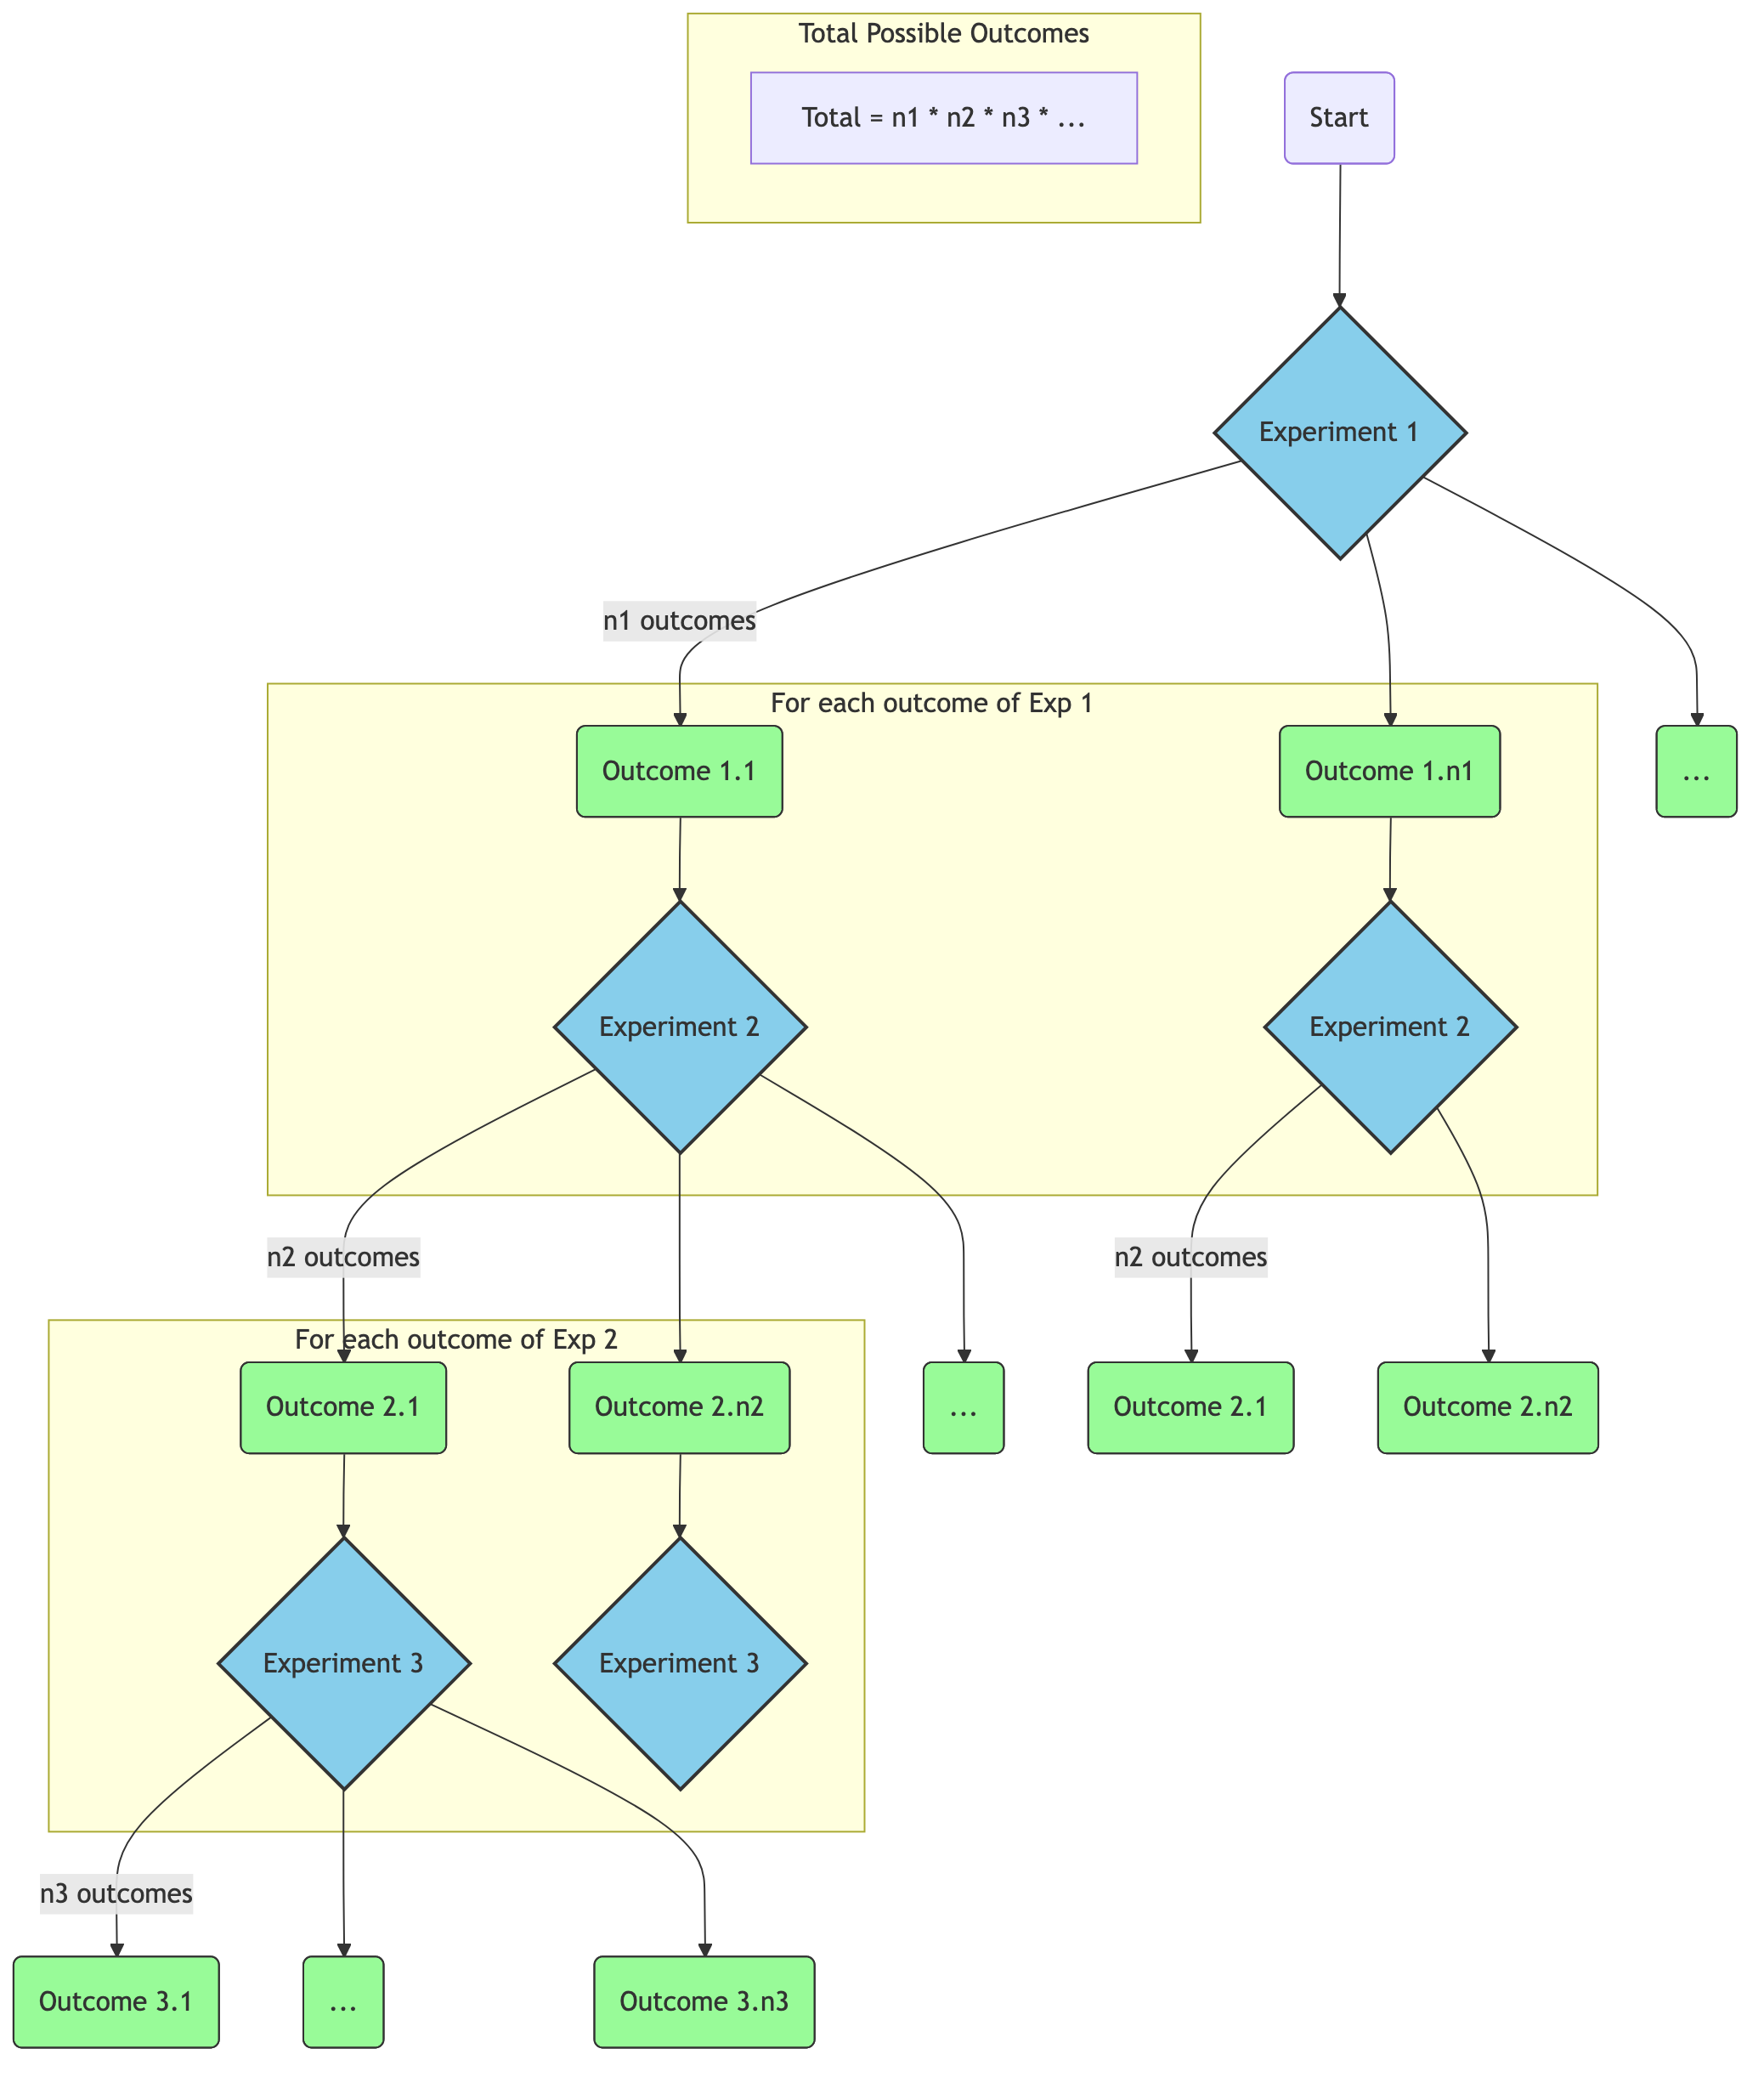
\includegraphics[width=0.8\textwidth]{counting.png}
    \caption{Mermaid diagram illustrating the Generalized Basic Principle of Counting}
    \label{fig:counting}
\end{figure}



\begin{examplebox}[title=Example: License Plates with Repetition]
    How many different \(7\) place license plates are possible if the first two places are to be occupied by letters and the remaining five by digits?
    
    \textbf{Solution:} The first two places can be filled with any of the \(26\) letters of the alphabet. Assuming letter can be repeated, the first place has \(26\) options and the second place has \(26\) options. The remaining five places can be filled with any of the \(10\) digits (from \(0\) to \(9\)), repeatedly. Therefore, the total number of different license plates is:

    \[
    26 \times 26 \times 10^5
    \]
\end{examplebox}

\begin{examplebox}[title=Example: License Plates without Repetition]
    If the letters and numbers in the previous example cannot be repeated, how many different license plates are possible?
    
    \textbf{Solution:} The first place has \(26\) options and the second place has \(25\) options (since letters cannot be repeated). The remaining five places can be filled with any of the \(10\) digits (from \(0\) to \(9\)). Therefore, the total number of different license plates is:

    \[
    26 \times 25 \times 10 \times 9 \times 8 \times 7 \times 6
    \]
\end{examplebox}

\section{Permutations}

\textbf{How many different ordered arrangements of letters \(a,b,c\) are possible?}

By enumeration we can see that : 

\[
abc, acb, bac, bca, cab, cba
\]
Each arrangement is called a \textbf{permutation} of the letters \(a,b,c\). There are \(6\) possible permutations for \(3\) distinct letters or a set of \(3\) distinct objects.

\begin{definitionbox}
    A permutation of \(n\) distinct objects is an arrangement of the objects in a specific order. The number of permutations of \(n\) distinct objects is given by \(n!\) (n factorial), which is the product of all positive integers up to \(n\):
    
    \[
    n! = n \times (n-1) \times (n-2) \times \ldots \times 2 \times 1
    \]
\end{definitionbox} 


\begin{examplebox}
    \textbf{Example 3:} How many different letter arrangments can be made from the letters PEPPER?
        \textbf{solution:} We have \(6\) letters in total where \(3\) letters are \(P\), \(2\) letters are \(E\) and \(1\) letter is \(R\). Therefore the number of different letter arrangements is given by:
        \[ \frac{6!}{3! \times 2! \times 1!} = 60 \]
        The idea is illustrated in Figure~\ref{fig:permute_pepper}.
\end{examplebox}

\begin{figure}[H!]
    \centering
    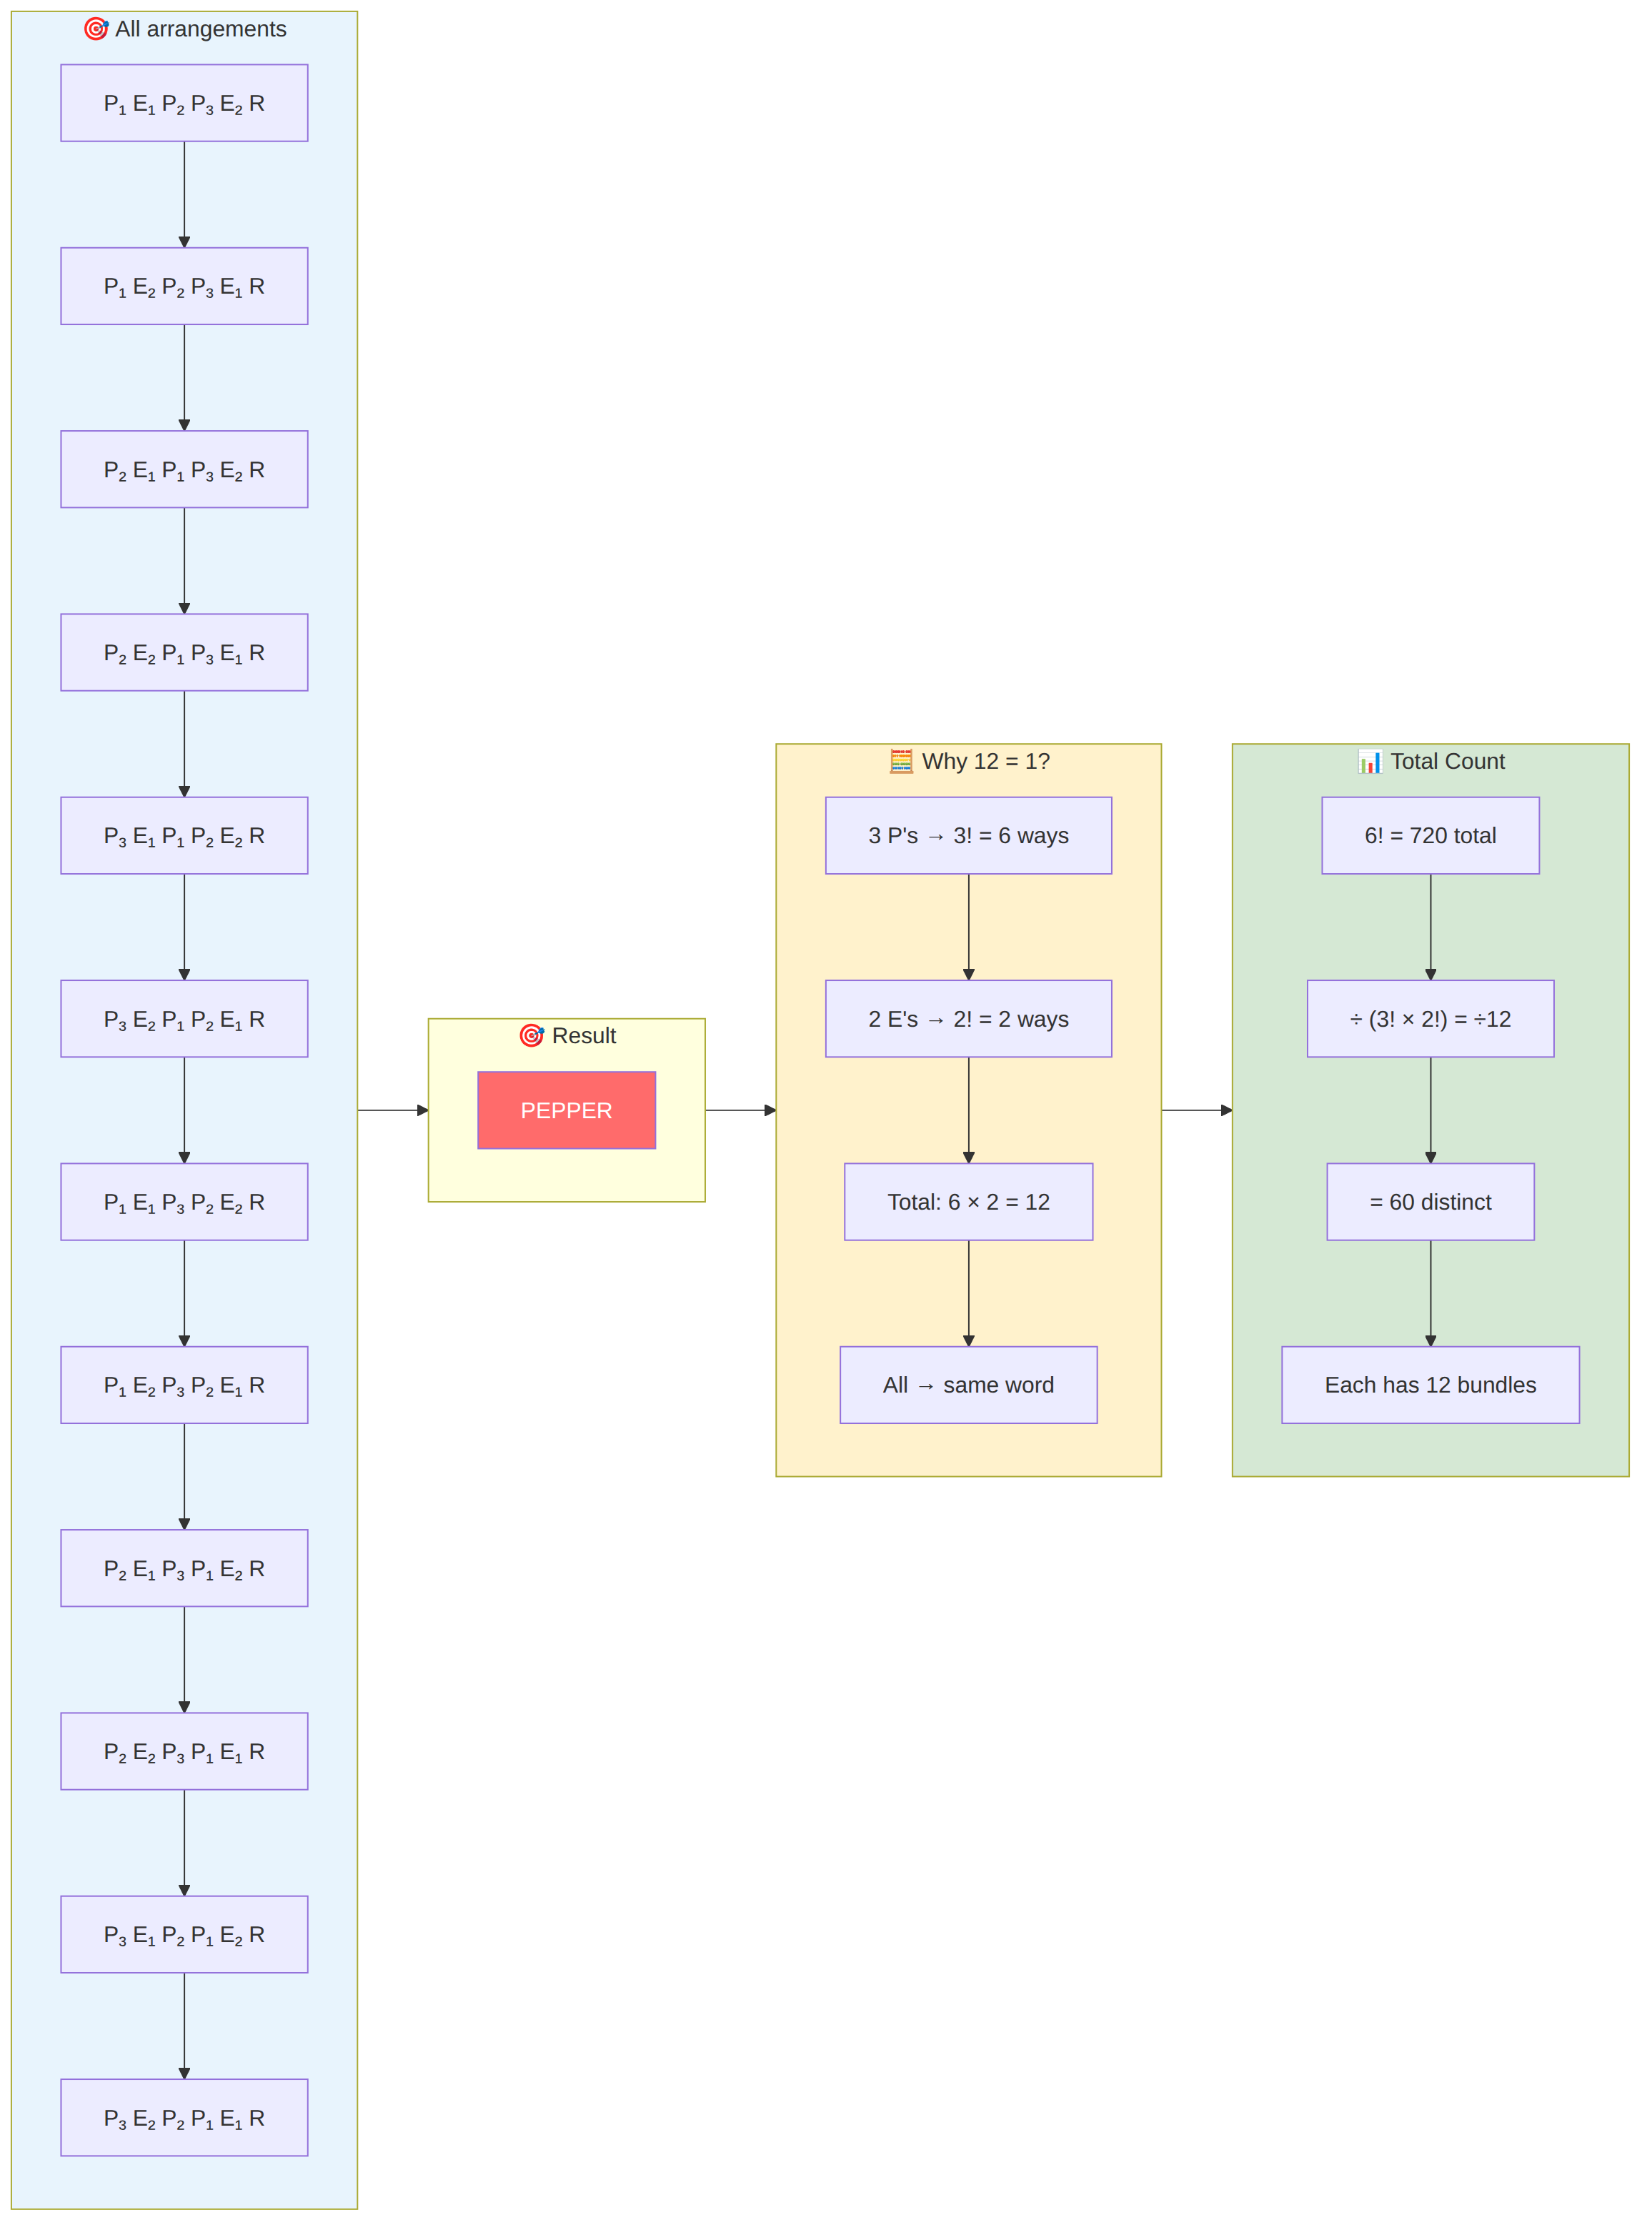
\includegraphics[width=1.1\textwidth]{permute_pepper_hd.png}
    \caption{The permutations of the letters in the word "PEPPER" by taking one permutation "PEPPER" and showing how many arrangements of the letters lead to the same word. This will repeat for other permutations as well}
    \label{fig:permute_pepper}
\end{figure}


\begin{keyconceptbox}
Let us start with \(n\) different objects and \(k\) be a positive integer such that \(k \leq n\). We want to determine the number of ways in which we can pick \(k\) objects from the total of \(n\) objects and arrange them in a sequence. i.e. the number of distinct \(k\) object sequence. We can do it in the following way 

\begin{itemize}
    \item We can pick the first object in \(n\) ways
    \item We can pick the second object in \(n-1\) ways (since we cannot pick the first object again)
    \item We can pick the third object in \(n-2\) ways (since we cannot pick the first and second objects again)
    \item ...
    \item We can pick the \(k\)-th object in \(n-(k-1)\) ways (since we cannot pick the first \(k-1\) objects again)
\end{itemize}

Therefore, by the generalized basic principle of counting, the total number of ways in which we can pick \(k\) objects from the total of \(n\) objects and arrange them in a sequence is given by
\[ 
    n \times (n-1) \times (n-2) \times \ldots \times (n-(k-1)) 
\]

\[
    = \frac{n(n-1)\cdots(n-(k-1))\times (n-k) \times (n-(k+1)) \times \cdots \times 2 \times 1}{(n-k) \times (n-(k+1)) \times \cdots \times 2 \times 1} 
\]

\[
= \frac{n!}{(n-k)!}
\]

In a special case when \(k=n\), we have
\[ \frac{n!}{(n-n)!} = \frac{n!}{0!} = n! \]
which is the number of ways in which we can arrange \(n\) distinct objects in a sequence.
\end{keyconceptbox}
\begin{exercisebox}
    \textbf{Exercise:} A chess tournament is to be held among \(10\) players. \(4\) are Russian, \(3\) are American, \(2\) are French and \(1\) is a German. How many different ways can the players be ranked from first to tenth place if the tournament just list the nationality of the players?
\end{exercisebox}


\begin{solutionbox}
    \textbf{Solution:} We have \(10\) players in total where \(4\) players are Russian, \(3\) players are American, \(2\) players are French and \(1\) player is German. Therefore the number of different ways the players can be ranked from first to tenth place is given by:
    \[ \frac{10!}{4! \times 3! \times 2! \times 1!} = 12600 \]
\end{solutionbox}

\section{Combinations}
\subsection{Inspiration}

Let's consider a problem: How many different groups of 3 objects could be formed from a total of 5 distinct objects A, B, C, D, and E?

If we think about selecting these objects in order, we'd have:
\begin{itemize}
    \item 5 ways to select the first object
    \item 4 ways to select the second object
    \item 3 ways to select the third object
\end{itemize}

Using the generalized basic principle of counting, we get $5 \times 4 \times 3 = 60$ ways of making ordered selections.

However, if we're only interested in which objects are in the group, not their order, then each distinct group is counted multiple times. For instance, the group \{A, B, C\} appears as all possible permutations: ABC, ACB, BAC, BCA, CAB, and CBA.

Since each group of 3 objects can be arranged in $3! = 6$ ways, the actual number of different groups is:
\[ \frac{5 \times 4 \times 3}{3!} = \frac{60}{6} = 10 \]

This illustrates the fundamental relationship between permutations and combinations: when we don't care about order, we divide the number of permutations by the number of ways to arrange the selected items.
\subsection{Definition}
\begin{definitionbox}
    A combination of \(n\) distinct objects taken \(r\) at a time is a selection of \(r\) objects from the total of \(n\) objects without regard to the order of selection. The number of combinations of \(n\) distinct objects taken \(r\) at a time is denoted by \(C(n,r)\) or \(\binom{n}{r}\) and is given by:
    
    \[
    C(n,r) = \binom{n}{r} = \frac{n!}{r!(n-r)!}
    \]
\end{definitionbox}

\begin{examplebox}[title=Example: Antennas with No Consecutive Defectives]
    \textbf{Problem:} Consider a set of $n$ antennas of which $m$ are defective and $n-m$ are functional. Assume that all defective antennas are indistinguishable from each other, and all functional antennas are indistinguishable from each other. How many linear orderings are there in which no two defective antennas are consecutive?
    
    \textbf{Solution:} This is a problem about combinations rather than permutations since we consider all defective antennas as identical, and likewise for functional antennas.
    
    To ensure no two defective antennas are consecutive, we need to place the $m$ defective antennas such that they are always separated by at least one functional antenna.
    
    Let's approach this by first placing the $n-m$ functional antennas in a row, creating $n-m+1$ potential positions for defective antennas (including before the first functional antenna, between functional antennas, and after the last functional antenna):
    
    \[
    \_ \circ \_ \circ \_ \circ \_ \cdots \circ \_
    \]
    
    where $\circ$ represents a functional antenna and $\_$ represents a potential position for defective antennas.
    
    Now, we need to choose $m$ positions out of these $n-m+1$ potential positions to place our defective antennas. This is a combination problem:
    
    \[
    \binom{n-m+1}{m} = \frac{(n-m+1)!}{m!(n-m+1-m)!} = \frac{(n-m+1)!}{m!(n-2m+1)!}
    \]
    
    Therefore, the number of linear orderings with no consecutive defective antennas is $\binom{n-m+1}{m}$.
    
    For example, if $n=7$ and $m=3$, then we have $\binom{7-3+1}{3} = \binom{5}{3} = 10$ possible arrangements with no consecutive defective antennas.
\end{examplebox}

\subsection{Pascal's Identity}
\begin{theorembox}[title=Pascal's Identity]
    For any integers \(n \geq 1\) and \(1 \leq k \leq n\),
    \[
    \binom{n}{k} = \binom{n-1}{k-1} + \binom{n-1}{k}
    \]
\end{theorembox}
\paragraph{Proof:}
We can prove Pascal's Identity using a combinatorial argument. Consider a set of \(n\) elements. We want to choose a subset of \(k\) elements from this set. We can do this in two ways:

1. **Case 1:** The first element is included in the subset. In this case, we need to choose \(k-1\) elements from the remaining \(n-1\) elements. The number of ways to do this is \(\binom{n-1}{k-1}\).

2. **Case 2:** The first element is not included in the subset. In this case, we need to choose \(k\) elements from the remaining \(n-1\) elements. The number of ways to do this is \(\binom{n-1}{k}\).

By considering both cases, we can express the total number of ways to choose \(k\) elements from \(n\) elements as the sum of the two cases:
\[
\binom{n}{k} = \binom{n-1}{k-1} + \binom{n-1}{k}
\]
This completes the proof of Pascal's Identity.

\subsubsection{Pascal's Triangle}
Pascal's Triangle is a triangular array of numbers where each number is the sum of the two directly above it. The \(n\)-th row corresponds to the coefficients in the expansion of \((x + y)^n\) and also represents the binomial coefficients \(\binom{n}{k}\).

\begin{figure}[h]
    \centering
    \begin{tabular}{ccccccccccc}
        & & & & & 1 & & & & & \\
        & & & & 1 & & 1 & & & & \\
        & & & 1 & & 2 & & 1 & & & \\
        & & 1 & & 3 & & 3 & & 1 & & \\
        & 1 & & 4 & & 6 & & 4 & & 1 & \\
        1 & & 5 & & 10 & & 10 & & 5 & & 1 \\
    \end{tabular}
    \caption{Pascal's Triangle showing the first 6 rows}
    \label{fig:pascal}
\end{figure}

\noindent
Each number in Pascal's Triangle is the sum of the two numbers above it. The value at position $(n,k)$ is $\binom{n}{k}$, where $n$ is the row number (starting from 0) and $k$ is the position within the row (also starting from 0).
\

\paragraph{The Connection:}
Pascal's Triangle is a direct visual representation of Pascal's Identity. The structure of the triangle is built using this identity as a fundamental rule. When constructing the triangle row by row, we start with 1 at the top and place 1's at both edges of each row (since $\binom{n}{0} = \binom{n}{n} = 1$). Every inner entry is then obtained by adding the two numbers directly above it—precisely following Pascal's Identity.

For example, examining row 4 ($n = 4$), the middle entry is $\binom{4}{2}$. By Pascal's Identity, this can be calculated as:
\[ \binom{4}{2} = \binom{3}{1} + \binom{3}{2} \]

Looking at the triangle, we can verify this: $3 + 3 = 6$, which is exactly the middle number in row 4. This pattern continues throughout the entire triangle, making it an elegant visual proof of Pascal's Identity and a useful tool for quickly calculating binomial coefficients.


\subsection{Binomial Theorm}
\begin{theorembox}[title=Binomial Theorem]
    For any integer \(n \geq 0\),
    \[
    (x + y)^n = \sum_{k=0}^{n} \binom{n}{k} x^{n-k} y^k
    \]
\end{theorembox}
\paragraph{Proof:}

\subsection{Binomial Theorem}
\begin{theorembox}[title=Binomial Theorem]
    For any positive integer \(n\),
    \[
    (x+y)^n = \sum_{k=0}^{n} \binom{n}{k} x^{n-k} y^k
    \]
\end{theorembox}
\paragraph{Proof:} Consider the product $(x+y)^n = \underbrace{(x+y)\,(x+y)\,\cdots\,(x+y)}_{\text{$n$ factors}}$.

When expanding this product, we must choose either $x$ or $y$ from each factor. To generate a term $x^{n-k}y^k$, we must select $y$ from exactly $k$ of the $n$ factors, and $x$ from the remaining $n-k$ factors.

The number of ways to select which $k$ factors contribute a $y$ is given by the binomial coefficient $\binom{n}{k}$. Thus, in the expansion, the coefficient of $x^{n-k}y^k$ is $\binom{n}{k}$.

Therefore:
\[
(x+y)^n = \sum_{k=0}^{n} \binom{n}{k}x^{n-k}y^k
\]

\begin{example}
For $n=3$:
\begin{itemize}[leftmargin=1.25em]
    \item $x^3$: choose $x$ from all factors (1 way)
    \item $x^2y$: choose $y$ from exactly 1 factor ($\binom{3}{1}=3$ ways)
    \item $xy^2$: choose $y$ from exactly 2 factors ($\binom{3}{2}=3$ ways)
    \item $y^3$: choose $y$ from all factors (1 way)
\end{itemize}

Thus $(x+y)^3 = x^3 + 3x^2y + 3xy^2 + y^3$, confirming the theorem.
\end{example}

\paragraph{Counting Principle Extension for Choosing Multiple Subsets}
We can extend our combinatorial principles to solve more complex problems, such as dividing a set into multiple groups. This directly connects to the concept of multinomial coefficients, which we'll explore next.

\subsection{Multinomial Coefficients}
\begin{definitionbox}[title=Multinomial Coefficient]
    Let $n$ and $r$ be positive integers, and let $n_1, n_2, \ldots, n_r$ be non-negative integers such that $n_1 + n_2 + \ldots + n_r = n$. The multinomial coefficient is defined as:
    \[
    \binom{n}{n_1, n_2, \ldots, n_r} = \frac{n!}{n_1! n_2! \cdots n_r!}
    \]
    
    This represents the number of ways to partition $n$ distinct objects into $r$ distinct groups, where group $i$ contains exactly $n_i$ objects.
\end{definitionbox}

\begin{examplebox}[title=Example: Committee Formation]
    A class of 20 students needs to form an executive committee with a president, vice president, secretary, and treasurer, and also needs to select 5 students for a planning committee and 6 students for a social committee. The remaining 5 students will not be on any committee. How many different ways can the committees be formed?
    
    \textbf{Solution:} This is a problem of partitioning 20 distinct students into 4 groups:
    \begin{itemize}
        \item 4 students for the executive committee
        \item 5 students for the planning committee
        \item 6 students for the social committee
        \item 5 students not on any committee
    \end{itemize}
    
    The number of ways to partition the students is:
    \[
    \binom{20}{4, 5, 6, 5} = \frac{20!}{4!5!6!5!} = 1,646,492,110,720
    \]
    
    However, within the executive committee, we must also assign specific roles. The 4 students can be arranged in $4! = 24$ ways. Therefore, the total number of different committee formations is:
    \[
    \frac{20!}{4!5!6!5!} \times 4! = \frac{20!}{5!6!5!} = 39,515,810,657,280
    \]
\end{examplebox}





\subsection{Multinomial Theorem}
\begin{theorembox}[title=Multinomial Theorem]
    For any positive integer \(n\) and any integer \(k \geq 2\),
    \[
    (x_1 + x_2 + \ldots + x_k)^n = \sum_{n_1+n_2+\ldots+n_k=n} \frac{n!}{n_1! n_2! \ldots n_k!} x_1^{n_1} x_2^{n_2} \ldots x_k^{n_k}
    \]
\end{theorembox}




\section{Applications of Combinatorial Analysis}
Combinatorial analysis has applications in various fields, including computer science, statistics, and operations research. Some common applications include:
\begin{itemize}
    \item Cryptography: Designing secure communication systems. For example, in RSA encryption, large prime numbers are used to create keys where the security relies on the computational difficulty of finding the prime factorization of large numbers.
    
    \item Network Design: Optimizing the layout of networks. For instance, determining the minimum number of routers needed to connect all computers in an office while minimizing cable length is a combinatorial optimization problem.
    
    \item Game Theory: Analyzing strategies in competitive situations. For example, in poker, calculating the probability of certain card combinations helps players make optimal betting decisions based on possible opponent hands.
    
    \item Probability Theory: Calculating probabilities in complex scenarios. For instance, in quality control, determining the probability of finding defective items in a batch using sampling techniques relies on combinatorial calculations.
\end{itemize}
